\section{Auswahl und Beschreibung der Messmethode}
\label{chap:auswahl_beschreibung_methode}

Während die CPU ein Programm ausführt, das aus einer Reihe von Befehlssätzen besteht, verbraucht sie unterschiedlich viel Strom. Die Idee der hier erstellten Messmethode ist es, ein Programm kontrolliert und mit präzis ausgewählten Befehlssätzen auf der CPU durchlaufen zu lassen. Das Programm in Form eines Benchmarks ist so konzipiert, dass ein bestimmter Befehlssatz millionenfach wiederholt wird. Dadurch wird der Stromverbrauch während der Ausführung über einen längeren Zeitraum konstant gehalten. Denn nur so ist eine aussagekräftige Messung möglich, da ein einzelner Befehlssatz so schnell durchläuft, dass er kaum messbar ist. Da die Ausführung der Befehlssätze wiederholt wird, muss die Messung durch die Anzahl der ausgeführten Wiederholungen geteilt werden.
\par
Die Strommessung erfolgt vom Leistungsverbrauch des ganzen Gerätes. Optimal wäre es, nur die Leistung der CPU zu messen. Dafür müsste aber die CPU vom Board ausgelötet und eine speziell dafür gebaute Messvorrichtung verwendet werden. Dazu kommt, dass nicht alle Datenblätter, welche die erforderliche Beschreibung und Belegung der Pins enthalten, für jedes Board oder für jeden Chip verfügbar sind. Deshalb wird ein SoC eingesetzt und die gesamte Leistung gemessen. SoC sind verfügbar auf kleinen Entwickler-Boards, die keine Lüfter, Laufwerke oder andere Verbraucher aufweisen, die hinsichtlich der Leistung störende Unregelmässigkeiten verursachen würden.



\begin{wrapfigure}{R}{0.6\textwidth}
\centering
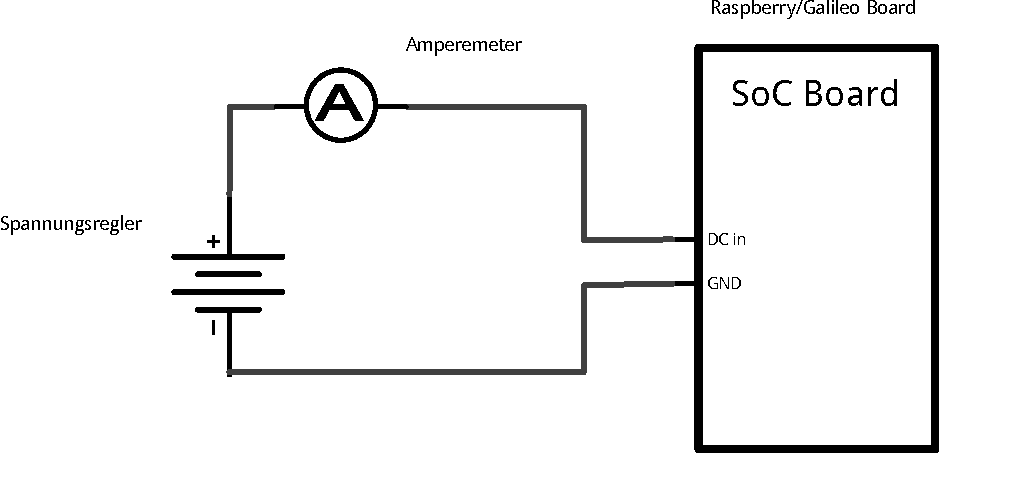
\includegraphics[scale=0.5]{images/schema.pdf}
\caption{Elektroschema für die Messung}
\label{fig:Elektroschema}
\end{wrapfigure}


Die für diese Arbeit verwendeten Boards werden im nächsten Kapitel im \autoref{beschreibung_hardware} beschrieben. Es wird davon ausgegangen, dass die Komponenten auf dem Board, abgesehen vom CPU selbst, während der Durchführung des Benchmarks vernachlässigbar kleine Leistungsschwankungen aufweisen. Die Messung erhält somit lediglich die Grundleistung der CPU, die vom Resultat abgezogen werden muss. Die Speisung erfolgt über einen Spannungsregler, der der Schaltung eine konstante Spannung liefert. Zwischen dem Spannungsregler und der Schaltung ist ein Amperemeter (Multimeter) zwischengeschaltet, der die Messung vornimmt. In der Abbildung \ref{fig:Elektroschema} ist das Elektroschema und die Platzierung des Amperemeters ersichtlich.
\par
Der eigentliche Kern des Benchmarks besteht aus gezielten und kurzen Assembler-Zeilen. Der Assemblercode bewirkt eine Schleife über einen zu testenden Befehlssatz. Damit das Ergebnis über einen längeren Zeitraum gemessen werden kann, wird der zu testende Befehlssatz einige Milliarden Mal wiederholt. So wird ein Zeitraum von zirka zwei bis drei Minuten erzeugt, in welchem die Messung auf einem der Prozessoren vorgenommen werden kann.
\par
Während dem Durchlaufen des Benchmarks darf die Ausführung nicht gestört werden. Jedes moderne Betriebssystem ist multitaskingfähig. Das bedeutet, dass das Betriebssystem eine Zeitscheibe besitzt und die Ressourcen der CPU abwechslungsweise an die Prozesse verteilt werden. Ein Benchmark darf also nicht als gewöhnlicher Prozess von einem Betriebssystem gestartet werden. Würde man das tun, hätte man keine Kontrolle, wann und wie viele Ressourcen der Benchmark schliesslich zugesprochen bekommt. Diese mangelnde Kontrolle würde das Messresultat verfälschen. Im Rahmen dieser Arbeit musste daher eine Methode erarbeitet werden, bei der der Benchmark während der Durchführung die vollen Ressourcen der CPU zugeteilt erhält und somit ein kontrollierter Ablauf garantiert ist.
\par
Die Ursprungsidee war es, direkt auf Baremetal zu arbeiten. Baremetal ist eine Ausdruck dafür, dass direkt auf der Hardware gearbeitet wird. Bei dieser Methode wird auf ein Betriebssystem verzichtet. Nach dem Bootprozess der Hardware wird ein Programm direkt gestartet und ausgeführt. An dieser Stelle wäre der Benchmark zum Zug gekommen. Eine speziell dafür präparierte Partition bootet die Hardware und führt den Benchmark aus.
\par
Für die Baremetal-Methode wurde ein funktionstüchtiger Prototyp erstellt. Es zeigten sich aber einige Nachteile. Auf komplexerer Hardware mit x86-Prozessoren ist der Boot-Vorgang um ein Vielfaches aufwendiger\cite{intel_boot_process}. Diese Prozessoren-Typen können nicht einfach beim Einschalten einen Programmcode ausführen. Es muss vorher eine lange Reihe von Abläufen in der Preboot Phase berücksichtigt und ausgeführt werden. Ein weiterer Nachteil der Baremetal-Methode ist die Überprüfung des Benchmarks. Die Gewährleistung, dass der Benchmark erwartungsgemäss funktioniert beziehungsweise überhaupt ausgeführt wird, benötigt ein Feedback nach aussen. Eine LED-Leuchte würde für dieses Feedback bereits ausreichen. Allerdings sind die GPIOs, die benötigt werden, um das LED zu steuern, je nach SoC sehr schwer anzusprechen, weil sie über einen PCI-Bus verbunden sind. Normalerweise stellt das Betriebssystem die nötigen C-Libraries zur Verfügung, um Komponenten, wie die GPIO, über einen PCI-Bus anzusteuern. Dieses fehlt hier jedoch gerade. Negativ wirkt sich zusätzlich die aufwendige Vorbereitung jedes einzelnen Tests aus. Für jeden Test muss eine Partition mit dem Benchmark erstellt und auf ein Medium kopiert werden. Damit die Messung erfolgen kann, muss dabei auch jedes Mal die Hardware neu gestartet werden. Unter diesen Umständen wird ein automatisierter Betrieb erheblich erschwert.
\par
Wegen der oben genannten Nachteile, wurde ein neues Konzept ausgearbeitet. Das neue Konzept arbeitet auf dem Betriebssystem Linux und bringt dadurch dessen Vorteile mit sich. Es muss sichergestellt werden, dass der Benchmark ohne Unterbrüche und abgeschirmt von anderen Prozessen durchgeführt wird. Um dies zu erreichen, wird der Benchmark anstatt im Benutzermodus (engl. User Space) im Kernelmodus (engl. Kernel Space) ausgeführt\cite{Mandl2010}. Der Programmcode, der innerhalb des Kernelmodus ausgeführt wird, muss als Kernelmodul kompiliert und im Kernel angemeldet werden. Schliesslich kann nur ein Interrupt den Code im Kernelmodul ausführen. Die genaue Beschreibung wird nachfolgend im \autoref{chap:benchmark_basis_interrupts} erläutert. Durch die Vornahme des Benchmarks im Kernelmodul werden alle Prozesse, die auf dem Betriebssystem parallel laufen, gestoppt und der Benchmark bekommt die vollen CPU-Ressourcen zugesprochen. In ein Kernelmodul können unterschiedliche Benchmarks gleichzeitig hinein kompiliert werden. Somit wird die Ausführung unterschiedlicher Tests vereinfacht. Dadurch wird eine spätere Automatisation ermöglicht, was zu einer Erleichterung der Messung beiträgt. 

 



 
